%!TEX root = thesis.tex
\chapter{Background}
\label{chapter:Background}

\textbf{Chapter Introduction}

\section{Vocabulary and Linguistics} % (fold)
\label{sec:vocabulary_and_linguistics}

\textbf{Might want to chuck language and linguistics intro in here}

\crumbs {

\textbf{Flow:}

- Vocabulary is a set of terms that a person is familiar with

- Vocabularies are expanded to describe new things we encounter

- By expanding our vocabularies we can be more expressive and precise with our communication

- However with the sheer volume of magnitude of terms that there are in language, it is beyond the capacity of humans to remember all of these terms

- So our brain will prioritise it's capacity to remember terms that are of most important and most frequent use to us

- While vocabularies are flexible in order to suit our needs...their development comes over time and it is not practical to uproot it all at once

}

Vocabulary is the set of words a person is familiar with in a given domain. This includes all terminology within the problem domain as well as the solution domain. Typically, this vocabulary grows and evolves in age and serves as a useful and fundamental tool for communication and acquiring knowledge.


\crumbs{We build vocabularies in order to more adequately and consistently describe things we encounter.}

\crumbs{Broadening vocabularies can allow us to be more expressive and precise with our communication.}

\crumbs{Humans don't quite have the capacity to expand their vocabularies to cover a language-worth of terms, so our brain will prioritise it's capacity to remember terms that are of most important and most frequent use to us.}

\crumbs{While vocabularies are flexible in order to suit our needs...their development comes over time and it is not practical to uproot it all at once}

\crumbs{What are the key components to building an effective natural language vocabulary?...how can these principles be applied to building other types of vocabularies?}

\crumbs{Linguistics play a role in our comprehension of something (how we relate to it/understand it with the building blocks we know)}

% \textbf{Need to be more effective selling the importance of vocabularies here}
% 
% \textbf{Will of course need citations of work studying how vocabulary is formed, the importance of vocabulary, how it changes, etc.}

% \crumbs{Vocabulary describes the collection of words that one has learnt and is able to recall.}

% \crumbs{But terms can be synonymous or polysemic depending upon context, meaning we have to choose our words carefully.}

% \crumbs{This allows to be more effective with our vocabularies}

% section vocabulary_and_linguistics (end)

\section{Source Code Vocabulary} % (fold)
\label{sec:source_code_vocabulary}

\crumbs{When it comes to source code vocabulary, there are very few boundaries regarding vocabulary}

\crumbs{We have conventions and idioms that are popular adhered to, but not enforced ... (getters, setters, general principles for naming things...)}

\crumbs{Problems addressed by software are so varied, that vocabularies will be different across different domains}

\crumbs{There is more to represent in source code vocabulary than just the terminology relating to the domain, etc, which begs the question? What exactly constitutes vocabulary in source code?}

\crumbs{Delorey \etal proposed a few definitions of vocabulary ... eventually settling on (one) because (the reason they chose)}

\crumbs{Delorey noted that we lack an adequate definition of vocabulary within the context of source code -- proposed levels at which we could define vocabulary...their study included just about everything as part of the vocabulary -- even operators}

\crumbs{Abebe et al. split the vocabulary across multiple levels of abstraction (class name, attribute name, method name, comment, etc.)}

\crumbs{
\textbf{Citable:}
Lexicon Bad Smells ... \cite{Abebe09b}
Analyzing the Evolution of the Source Code Vocabulary \cite{Abebe09a}
Mining Programming Language Vocabularies From Source Code \cite{Delorey09a}
The Programmer's Lexicon \cite{Host07a}
}

% section source_code_vocabulary (end)

\section{Mental Models} % (fold)
\label{sec:mental_models}

\crumbs{Mental models describe our cognitive process in regard to comprehension of things we are exposed to}

\crumbs{We build mental models as they allow us an understanding of something that is more akin to each individuals way of thinking}

\crumbs{Team mental models are important, so that team members comprehensions of something are not wildly different (though not all the same -- different perspectives can be a good thing...) -- need to have a consistent representation of a problem if they are to work towards to a well-formed solution.}

\crumbs{Languages play a significant role in building mental models, as we as humans associate our understanding with something using the language we have acquired that can be used to describe it.}

% section mental_models (end)

\section{Software Mental Models} % (fold)
\label{sec:software_mental_models}

% TODO: Should cite work on users mental models of software...Don't Make Me Think? Find some good HCI stuff for here

\draft{Software systems are complex entities, rich with conceptual information relating to the domain in which it operates and the problems it attempts to solve \cite{Biggerstaff93a}. Users of software face the challenges of establishing adequate comprehension of what a piece of software is designed to do and how it aligns with what they want it to do. Accordingly, users must develop a mental model of the software in order for it to be useful for their purpose.}

% TODO: Need a citation for OO and design patterns being closely related to natural patterns of thinking

\draft{Developers have the responsibly of not only understanding how the software works, but also to communicate to a computer how it should behave and to other developers how it is constructed. Fortunately, developers are able to rely heavily on real-world objects and metaphors in communicating to other developers how a software system has been built. The use of programming paradigms such as object-oriented programming and design patterns allow a cognitive map for developers to apply traditional thinking within a software context. However, this freedom of expression is a double-edged sword, as developers are by no means obliged to be communicative when writing code.}

\crumbs{Concepts, domain terms}

\draft{Numerous studies have investigated the quality of identifiers within source code \cite{Abebe09b,Caprile00a,Caprile99a,Deissenboeck06a,Lawrie06a,Lawrie06b,Lawrie07a,Takang96a}. In \cite{Deissenboeck06a}, Dei{\ss}enb\"{o}ck and Pizka define a formal model for well-formed identifiers, with rules for \emph{concise} and \emph{consistent} naming. Lawrie \etal perform an empirical investigation of 78 systems based upon this model to determine whether programmers conform to these rules in their code, revealing that developers frequently violated these rules \textbf{TODO: How frequently? Need some numbers here}. Lawrie \etal examine the impact of identifier completeness upon the comprehension of developers \cite{Lawrie06a}. In their study, they assess the ability of over 100 developers to comprehend function identifiers at three different levels of completeness --- \emph{single letters}, \emph{abbreviations}, and \emph{full words} --- based on well-known algorithms and production code samples. Their study showed that full word identifiers lead to the highest level of comprehension, although in a lot of cases the difference between abbreviation and full word identifiers was negligible.}

% section software_mental_models (end)

\section{Natural Language vs. Programmer Language} % (fold)
\label{sec:natural_language_vs_programmer_language}

\begin{figure}[t]
\centering
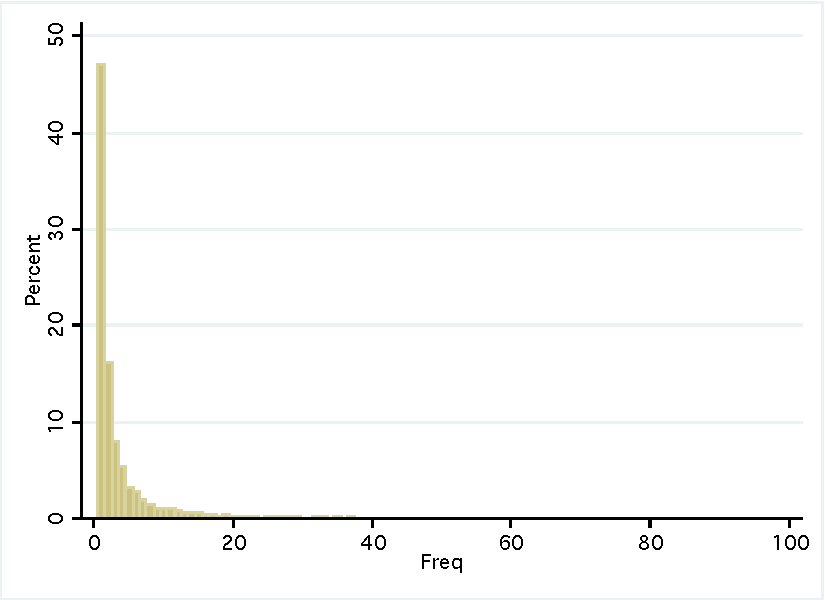
\includegraphics[width=\textwidth]{Figures/Vocab-GadflyFreqDist.pdf}
\caption{Term frequency distribution for \emph{The Gadfly}, showing a preference towards using a large number of terms infrequently}
\label{fig:vocab-freqdist-gadfly}
\end{figure}

\crumbs{\textbf{Citable:} Corpus Linguistics ... \cite{Biber98a} 
Corpus Linguistics ... \cite{McEnery01a}
Selective Studies (Zipf) \cite{Zipf49a}}

\crumbs{Studies of natural language/corpus linguistics have shown us that there are tendencies for humans to apply language in a particular way within natural language documents.}

\crumbs{These studies have allowed us to develop ways in which we can assist in the production of text corpora (how?)}

\crumbs{Lots of studies have been undertaken in the field of natural language. These studies have been effective in providing an understanding of how humans learn, process and use language.}

\crumbs{Programming Languages, Natural Languages and Mathematics ... \cite{Naur75a}}

\crumbs{While programs are written using terms that are close to that of natural language, there is little knowledge as to whether the two are exactly the same.}

\crumbs{Mining Programming Vocabularies ... \cite{Delorey09a}}

\crumbs{An Empirical Exploration of Regularities in Open-Source Software Lexicons ...\cite{Pierret09a}}

\crumbs{However, we suspect that there are some similarities between the two which would allow us to apply what we know of natural language to programmer languages}
 
\crumbs{Investigation of the similarities between the language used in source code and the language used in natural language corpora indicate that there are definite similarities between the two, opening the door for the possibility of the application of natural language analysis techniques to source code.}

\crumbs{Outline studies that have investigated the similarities between the two, what success they had and what they claimed it could yield}

% section natural_language_vs_programmer_language (end)

% \section{Software Evolution} % (fold)
% \label{sec:software_evolution}
% 
% % section software_evolution (end)

\section{Source Code Vocabulary Evolution} % (fold)
\label{sec:source_code_vocabulary_evolution}

\draft{While there have been numerous studies that have investigated the nature of evolution of source code within software systems, which have given an idea of what to expect through various stages of evolution \textbf{(Cite some!)}; what is unclear is how the vocabulary that is captured within the source code evolves, as the system itself evolves.}

\draft{It would be reasonable to assume that --- given the vocabulary of the source code is a core part of the source code itself --- it would be subject to the same evolutionary pressures. Antoniol \etal compared the evolution of the source vocabulary and that of the program structure \cite{Antoniol07a}, with a particular focus on their stability. Their study found that the vocabulary (or \emph{lexicon}, as they referred to it) exhibited a high level of stability --- higher than that of the program structure for all versions of the software systems they analysed. While they were able to find a correlation between the two, with major changes in structure yield similarly significant changes in the lexicon, they noted that the underlying distributions between the two were statistically different.}

\draft{\cite{Antoniol07a} also investigated the frequency of changes to program entities (methods/functions) resultant from identifier refactoring, with the results showing that changes to the lexicon brought about via renaming are very rare, implying developers are hesitant to alter the names of entities within a program once they have been put in place. They speculate that this is due to a reluctance of developers to bring about substantial changes to their mental model of the software.}

\crumbs{Abebe \etal \cite{Abebe09a} found that the size of the system and the vocabulary exhibit similarities in their evolution.}

\draft{Their study established separate vocabularies for the different levels of abstraction within source code, including \emph{class name}, \emph{attribute name}, \emph{function name}, \emph{parameter name} and \emph{comment} vocabularies. Interestingly, they found that of the vocabularies they had established, the comment vocabulary was the largest contributor to evolution of the vocabulary and rich in representation of the entire vocabulary, containing over $ \frac{3}{4} $ of the terms found in any of the vocabularies.}

\draft{Additionally, they investigated the introduction of new identifiers within a release, to determine whether they were bringing about new terms or whether there was a tendency towards re-use of existing terms. Their findings were that new identifiers consisted of only existing terms in 56\% percent and 70\% of cases for ALICE and WinMerge respectively.}

% section source_code_vocabulary_evolution (end)

\section{Summary} % (fold)
\label{sec:summary}

\crumbs{Summarise current state of research that is most closely related to this thesis and highlight the gaps}

\crumbs{Outline how our research fits in and how it addresses those gaps}

% section summary (end)

\section{Research Questions} % (fold)
\label{sec:research_questions}

\begin{itemize}
	% Growth-related questions
	\item What are the trends for growth in total size of the vocabulary across evolving software systems? Does this match findings for the growth of software systems as a whole?
	% Distribution-related questions
	\item What is the distribution of term usage frequency within vocabulary?
		\begin{itemize}
			\item Is there an observable similarity in the vocabulary distribution profiles between systems?
		\end{itemize}
	\item How does the distribution of term usage change throughout the evolution of a system?
		\begin{itemize}
			\item Are the most popular continually re-used?
			\item Are changes to the vocabulary stable or erratic?
		\end{itemize}
	\item Does the age of a term have an influence on the likelihood that it will be re-used?
	\item What do the most frequently used terms refer to? Are these terms related to the domain or architectural concepts (such as idioms and design patterns)?
\end{itemize}

% section research_questions (end)